% !TEX program = xelatex
% =============================================================================
% 中文求职简历 LaTeX 模板
% Author: Kody
% Repository: https://github.com/kodyyu1126/Chinese-resume-template-work
% Compiler: XeLaTeX
%
% 快速修改指南：
% 1. 在“个人信息头部”中替换姓名、联系方式、求职意向和头像。
% 2. 在“教育背景”中替换学校、专业、成绩排名和课程信息。
% 3. 在实习经历、项目经历、校园经历与荣誉技能模块中增删示例内容。
% 4. 如需调整样式，可修改下方的字体、页面边距与 sectioncolor 配置。
% =============================================================================
\documentclass[11pt,a4paper,fontset=none]{ctexart}

% ── 字体设置 ──────────────────────────────────────────────
% 若需在 Overleaf 使用自定义字体，可将已授权的字体文件放入 fonts/ 文件夹，
% 并按 STSong.ttf、STHeiti.ttf、STKaiti.ttf 命名；macOS 本地默认使用系统华文系列。
\IfFontExistsTF{Times New Roman}{\setmainfont{Times New Roman}}{}

\newif\ifuseuploadedcjkfonts
\IfFileExists{fonts/STSong.ttf}{
    \IfFileExists{fonts/STHeiti.ttf}{
        \IfFileExists{fonts/STKaiti.ttf}{\useuploadedcjkfontstrue}{}
    }{}
}{}

\newif\ifusesystemcjkfonts
\IfFontExistsTF{STSong}{
    \IfFontExistsTF{STHeiti}{
        \IfFontExistsTF{STKaiti}{\usesystemcjkfontstrue}{}
    }{}
}{}

\ifuseuploadedcjkfonts
    \setCJKmainfont[
        Path = fonts/,
        BoldFont = STHeiti.ttf,
        ItalicFont = STKaiti.ttf
    ]{STSong.ttf}
    \setCJKsansfont[Path = fonts/]{STHeiti.ttf}
    \setCJKmonofont[Path = fonts/]{STHeiti.ttf}
\else\ifusesystemcjkfonts
    \setCJKmainfont[
        BoldFont = STHeiti,
        ItalicFont = STKaiti
    ]{STSong}
    \setCJKsansfont{STHeiti}
    \setCJKmonofont{STHeiti}
\else
    \IfFontExistsTF{KaiTi}{
        % Windows 中文楷体（正文、标题、粗体统一使用楷体；AutoFakeBold 模拟加粗，使 \textbf 可见）
        \setCJKmainfont[AutoFakeBold = 2.5, ItalicFont = KaiTi]{KaiTi}
        \setCJKsansfont{KaiTi}
        \setCJKmonofont{KaiTi}
    }{
        \setCJKmainfont[
            BoldFont = Noto Sans CJK SC,
            ItalicFont = Noto Serif CJK SC
        ]{Noto Serif CJK SC}
        \setCJKsansfont{Noto Sans CJK SC}
        \setCJKmonofont{Noto Sans CJK SC}
    }
\fi
\fi

% ── 页面布局 ──────────────────────────────────────────────
\usepackage{geometry}
\geometry{a4paper, left=1.5cm, right=1.5cm, top=1.5cm, bottom=1.5cm}

% ── 颜色定义 ──────────────────────────────────────────────
\usepackage{xcolor}
\definecolor{sectioncolor}{RGB}{46,116,181}
\definecolor{linkcolor}{RGB}{0,112,192}
\definecolor{textcolor}{RGB}{0,0,0}

% ── 标题格式 ──────────────────────────────────────────────
\usepackage{titlesec}
\titleformat{\section}
    {\Large\bfseries\color{sectioncolor}}
    {}
    {0em}
    {\uppercase}
    [\vspace{-0.8em}\rule{\textwidth}{1pt}]
\titlespacing{\section}{0pt}{0.1em}{0.05em}

% ── 列表格式 ──────────────────────────────────────────────
\usepackage{enumitem}
\setlist[itemize]{leftmargin=*, nosep, topsep=0.2em, itemsep=0.1em, parsep=0em}

% ── 图片与排版 ────────────────────────────────────────────
\usepackage{graphicx}
\setkeys{Gin}{draft=false}
\usepackage[export]{adjustbox}
\usepackage{calc}

% ── 表格 ─────────────────────────────────────────────────
\usepackage{tabularx}
\usepackage{multirow}

% ── 图标与超链接 ──────────────────────────────────────────
\usepackage{fontawesome5}
\usepackage{hyperref}
\hypersetup{colorlinks=true, linkcolor=linkcolor, urlcolor=linkcolor}

% ── 全局样式 ──────────────────────────────────────────────
\color{textcolor}
\linespread{1.06}
\setlength{\parindent}{0pt}
\pagestyle{empty}

% ── 自定义命令 ────────────────────────────────────────────
\newcommand{\daterange}[1]{{\textbf{#1}}}
\newcommand{\entrytitle}[1]{{\textbf{#1}}}
% 内容条目：无序列表样式（空心圆点顶格 + 悬挂缩进），换行自动对齐
\newcommand{\rinfo}[1]{\begin{itemize}[leftmargin=1.2em, labelindent=0pt, labelwidth=0.7em, labelsep=0.5em, itemindent=0pt, label=$\circ$, nosep, topsep=0.15em, itemsep=0em, parsep=0em, partopsep=0em]\item #1\end{itemize}}

% ============================================================
\begin{document}
\setlength{\parindent}{0pt}
% ============================================================

% ── 个人信息头部：照片 + 姓名信息 + 二维码 ──
\vspace*{-1.2em}
% 将信息区装入盒子并测量其总高度，用于统一照片与二维码的高度
\newsavebox{\headinfobox}
\begin{lrbox}{\headinfobox}%
\begin{tabular}{@{}l@{}}
    {\Huge\bfseries 张皓琛} \\[0.7em]
    出生年月日：2002.10.06 \\[0.25em]
    电话：19198026326 \\[0.25em]
    邮箱：holden4study@gmail.com
\end{tabular}%
\end{lrbox}
\newlength{\headh}
\setlength{\headh}{\ht\headinfobox}%
\addtolength{\headh}{\dp\headinfobox}%
% 二维码高度（保持不变）
\newlength{\photoh}
\setlength{\photoh}{1.0\headh}
% 仅头像使用的高度：比二维码/信息区略大，只放大照片
\newlength{\profileh}
\setlength{\profileh}{1.1\headh}
% 照片栏宽度贴合放大后的照片；再量出原尺寸宽度，用于抵消照片变宽对信息区位置的影响
\newlength{\photow}
\settowidth{\photow}{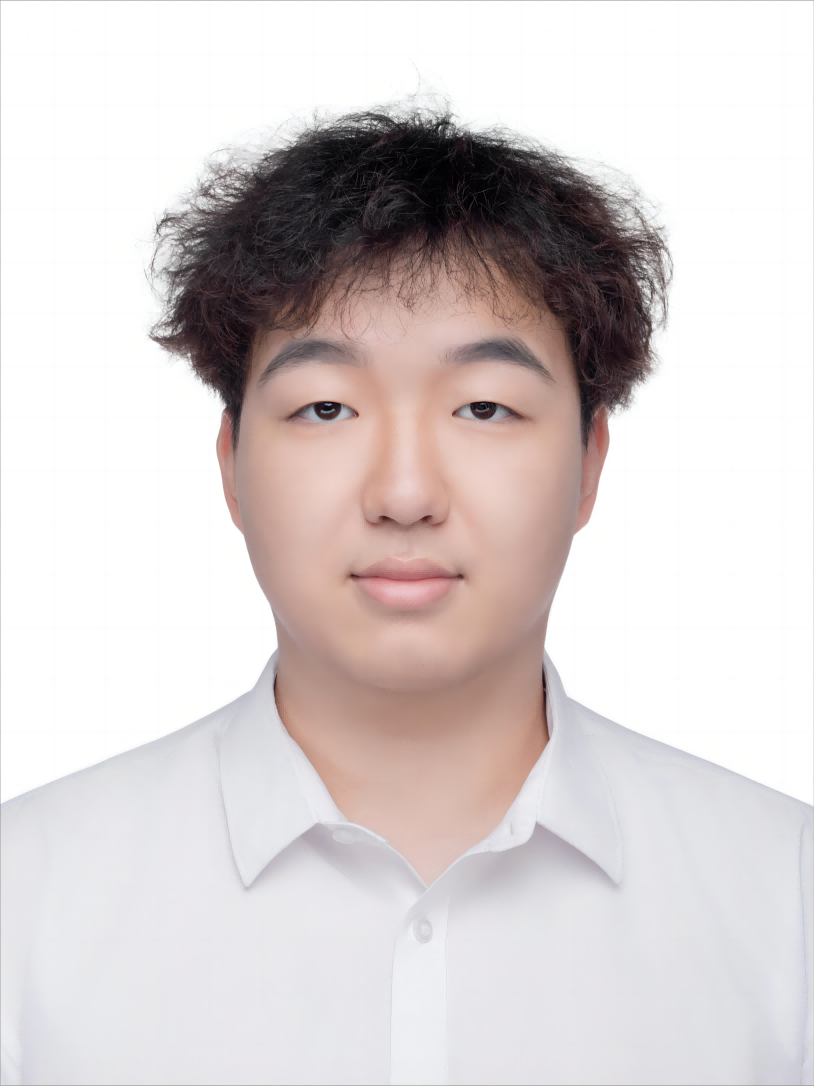
\includegraphics[height=\profileh]{assets/profile-photo.png}}
\newlength{\oldphotow}
\settowidth{\oldphotow}{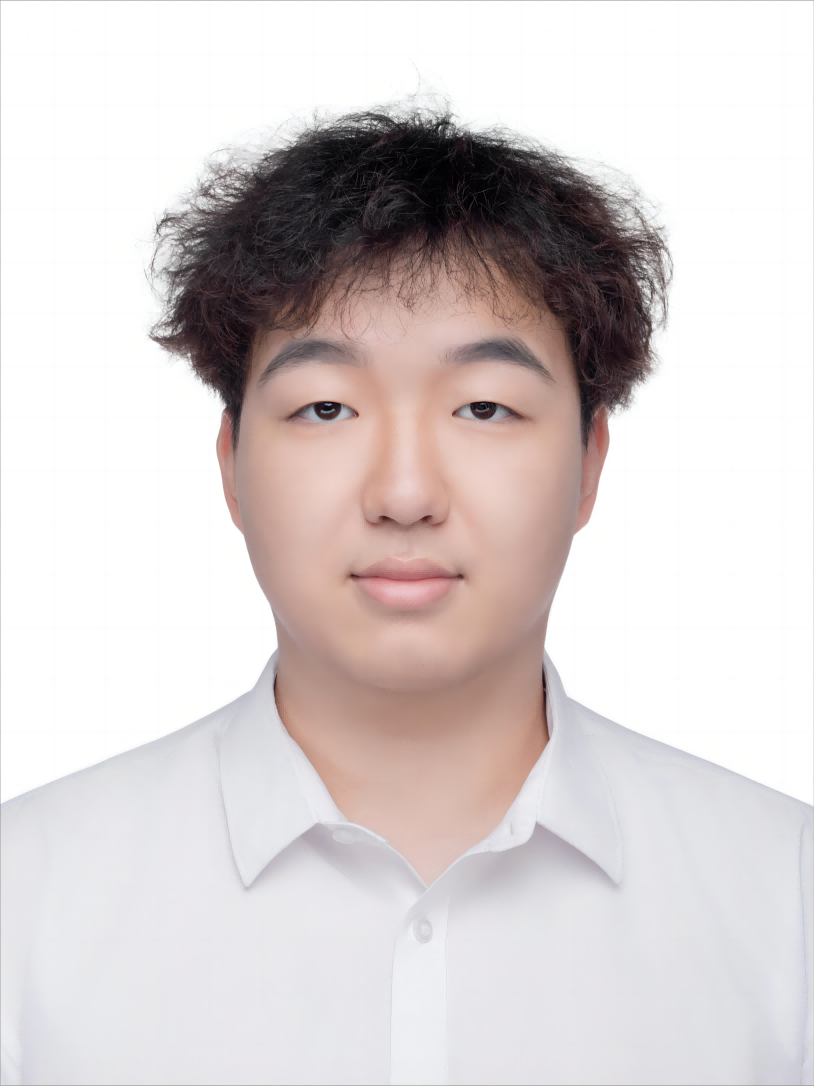
\includegraphics[height=\photoh]{assets/profile-photo.png}}
% 二维码为正方形：栏宽等于二维码整图宽度，使“个人主页”居中于二维码正下方
\newlength{\qrw}
\setlength{\qrw}{\photoh}
% 整行强制为文本宽度：照片贴左边界，二维码靠右并留出一点右边距
\noindent\hbox to \textwidth{%
\begin{minipage}[t]{\photow}
    \setlength{\parindent}{0pt}%
    \vspace*{-0.15\headh}
    \raggedright
    % 头像：替换为自己的图片（仅此高度放大）
    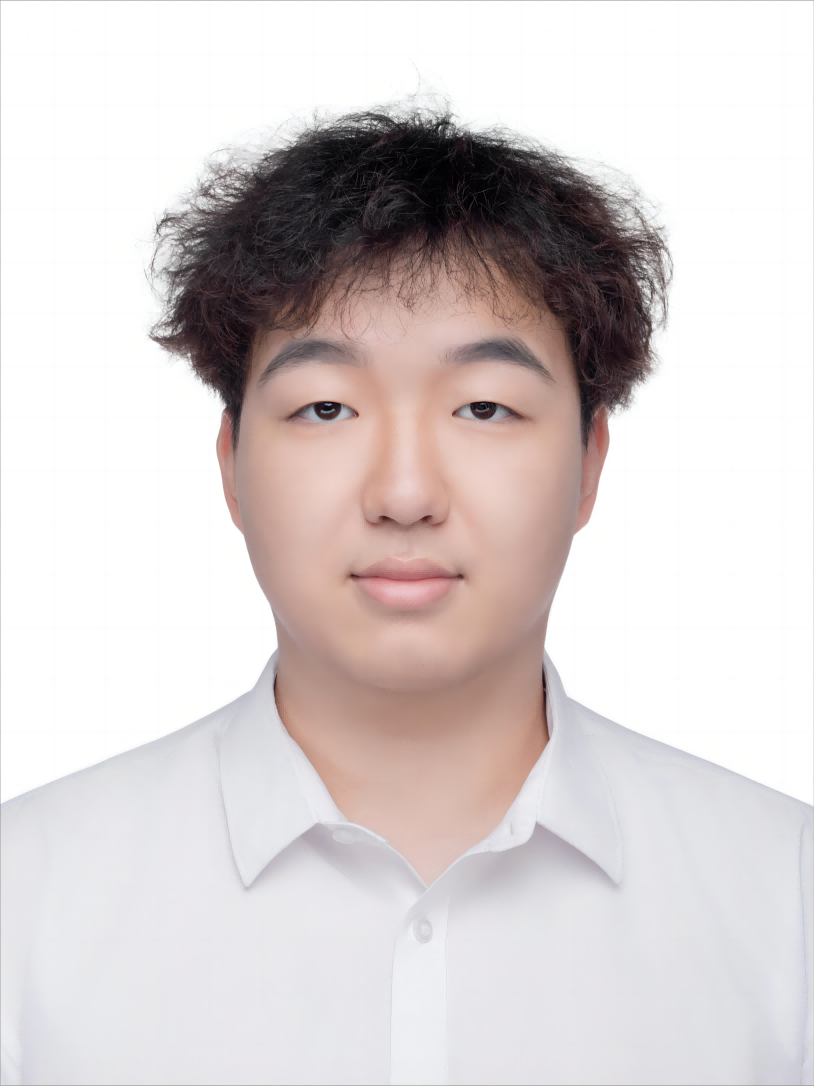
\includegraphics[height=\profileh,keepaspectratio]{assets/profile-photo.png}
\end{minipage}%
\hspace{\dimexpr 1em-\photow+\oldphotow\relax}%
\begin{minipage}[t]{0.5\textwidth}
    \setlength{\parindent}{0pt}%
    \vspace{0pt}
    \usebox{\headinfobox}
\end{minipage}%
\hfil
\begin{minipage}[t]{\qrw}
    \setlength{\parindent}{0pt}%
    \vspace*{-0.05\headh}
    \centering
    % 个人主页二维码（指向中文主页 https://zhang-holden.github.io/zh/）；文字与“邮箱”同号，紧贴二维码下方
    
\includegraphics[height=\photoh,keepaspectratio]{assets/qr-zh.png}\\[\dimexpr 0.2em-5pt\relax]
    个人主页
\end{minipage}%
\hspace{5.6pt}%
}%

\vspace{\dimexpr 0.8em-3pt\relax}

% ── 教育背景：替换学校、专业、时间、GPA、排名和主修课程 ──
\section*{教育背景}
\vspace{-0.2em}

\noindent
\textbf{长沙理工大学}\hfill\textbf{工程管理（学士）}\hfill\textbf{2020.09 \textasciitilde{} 2024.06}

\rinfo{主修课程：道路工程、桥梁工程、工程项目管理、工程财务管理、工程风险管理与保险、公路工程造价、FIDIC条件与合同管理、BIM技术及应用等。}

\vspace{0.2em}

\noindent
\textbf{新西兰奥克兰大学}\hfill\textbf{基础设施资产管理（研究型硕士）}\hfill\textbf{2025.04 \textasciitilde{} 2026.12}

\rinfo{主修课程：基础设施资产管理、大数据管理、智能基础设施分析、基础设施的气候韧性分析、全生命周期评估方法等。}

% ── 研究经历：About 页面研究内容（时间待补充）──
\section*{研究经历}
\vspace{-0.1em}

\noindent
\textbf{绿色道路养护决策的双层优化方法研究}\hfill{}\textbf{本科毕业论文}

\rinfo{研究概述：构建低碳背景下道路养护决策的双层优化模型，以 Python 为编程语言开发多目标优化算法，在碳排放、养护成本与路面性能等指标间寻求最优平衡；论文摘要被 2024 年世界交通运输大会（WTC）收录并做现场海报汇报。}

\vspace{0.2em}

\noindent
\textbf{电动汽车充电基础设施碳资产化框架研究}\hfill{}\textbf{硕士毕业论文}

\rinfo{研究概述：利用区块链技术，并用 Solidity 语言开发智能合约，构建覆盖建设、运营、维护、报废各阶段的电动汽车充电基础设施全生命周期碳追踪与资产化框架，实现碳足迹的全过程可信追踪，为碳减排成果转化为可交易的碳信用提供技术保障。}

\vspace{0.2em}

\noindent
\textbf{再生面粉产品全生命周期评价}\hfill{}\textbf{硕士研究项目}

\rinfo{研究概述：作为研究小组成员，与新西兰环保企业 Rescued Kitchen 合作，基于全生命周期评价（LCA）方法框架，使用 OpenLCA 对产品从原料到成品全过程的环境影响进行量化评估，识别主要环境影响并提出改进方向；研究成果向企业联合创始人汇报，并被奥克兰大学官网新闻及新西兰晨间新闻报道。}

\vspace{0.2em}

\noindent
\textbf{奥克兰 Mission Bay 海岸线内基础设施气候适应研究}\hfill{}\textbf{硕士研究项目}

\rinfo{研究概述：针对奥克兰 Mission Bay 海岸线内的基础设施，运用奥克兰市议会灾害情景模拟工具，分析海平面上升、风暴潮等多种灾害情景下的海岸淹没与侵蚀影响，提出分阶段适应性改造策略，为沿海基础设施的气候韧性规划提供决策依据。}

% ── 校园经历 ──────────────────────────────────────────────
\section*{校园经历}
\vspace{-0.1em}

\noindent
\textbf{长沙理工大学}\hfill\textbf{交通运输工程学院篮球队队员}

\vspace{0.2em}
\noindent
\textbf{长沙理工大学}\hfill\textbf{校篮协裁判委员会主任}

\rinfo{主要职责：负责校篮协成员的裁判培训，并与市篮协对接，组织校篮协成员裁判证考试相关事宜；执裁院级、校级以及长沙市 NYBO 小篮球比赛；负责湘煤集团、省直机关篮球比赛的记录台工作。}

\vspace{0.2em}
\noindent
\textbf{长沙理工大学}\hfill\textbf{阳光书屋办公室副主任}

\rinfo{主要职责：负责书籍借阅和库存管理相关工作，并协调安排值班人员，制定排班计划。}

\vspace{0.2em}

\noindent
\textbf{新西兰奥克兰大学}\hfill\textbf{篮球俱乐部成员}

\rinfo{主要职责：参与校篮球俱乐部相关活动，并执裁相关篮球赛事。}

% ── 技能资格 ──────────────────────────────────────────────
\section*{技能资格}
\vspace{-0.1em}
\rinfo{语言能力：CET-6、奥克兰大学学术英语证书。}

\rinfo{编程与数据：Python、Solidity、XML、XPath、XQuery、LaTex。}

\rinfo{工程软件：Revit、AutoCAD、OpenLCA。}

\rinfo{其他：二级篮球裁判员、新西兰 Level-1 篮球裁判员。}

\end{document}
